\documentclass{standalone}
\usepackage{tikz}
\usepackage{tikz-cd}
\usepackage{tikz-3dplot}
\usepackage{pgfplots}
\usepackage{pgffor} % For \foreach loop
\pgfplotsset{compat=newest} % Adjust to your version of pgfplots
\def\Circlearrowleft{\ensuremath{%
		\rotatebox[origin=c]{180}{$\circlearrowleft$}}}
\def\Circlearrowright{\ensuremath{%
		\rotatebox[origin=c]{180}{$\circlearrowright$}}}
\def\CircleArrowleft{\ensuremath{%
		\reflectbox{\rotatebox[origin=c]{180}{$\circlearrowleft$}}}}
\def\CircleArrowright{\ensuremath{%
		\reflectbox{\rotatebox[origin=c]{180}{$\circlearrowright$}}}}
\usetikzlibrary{
	3d, % For 3D drawing
	angles,
	arrows,
	arrows.meta,
	backgrounds,
	bending,
	calc,
	decorations.pathmorphing,
	decorations.pathreplacing,
	decorations.markings,
	fit,
	matrix,
	patterns,
	patterns.meta,
	positioning,
	quotes,
	shadows,
	shapes,
	shapes.geometric
}

\begin{document}
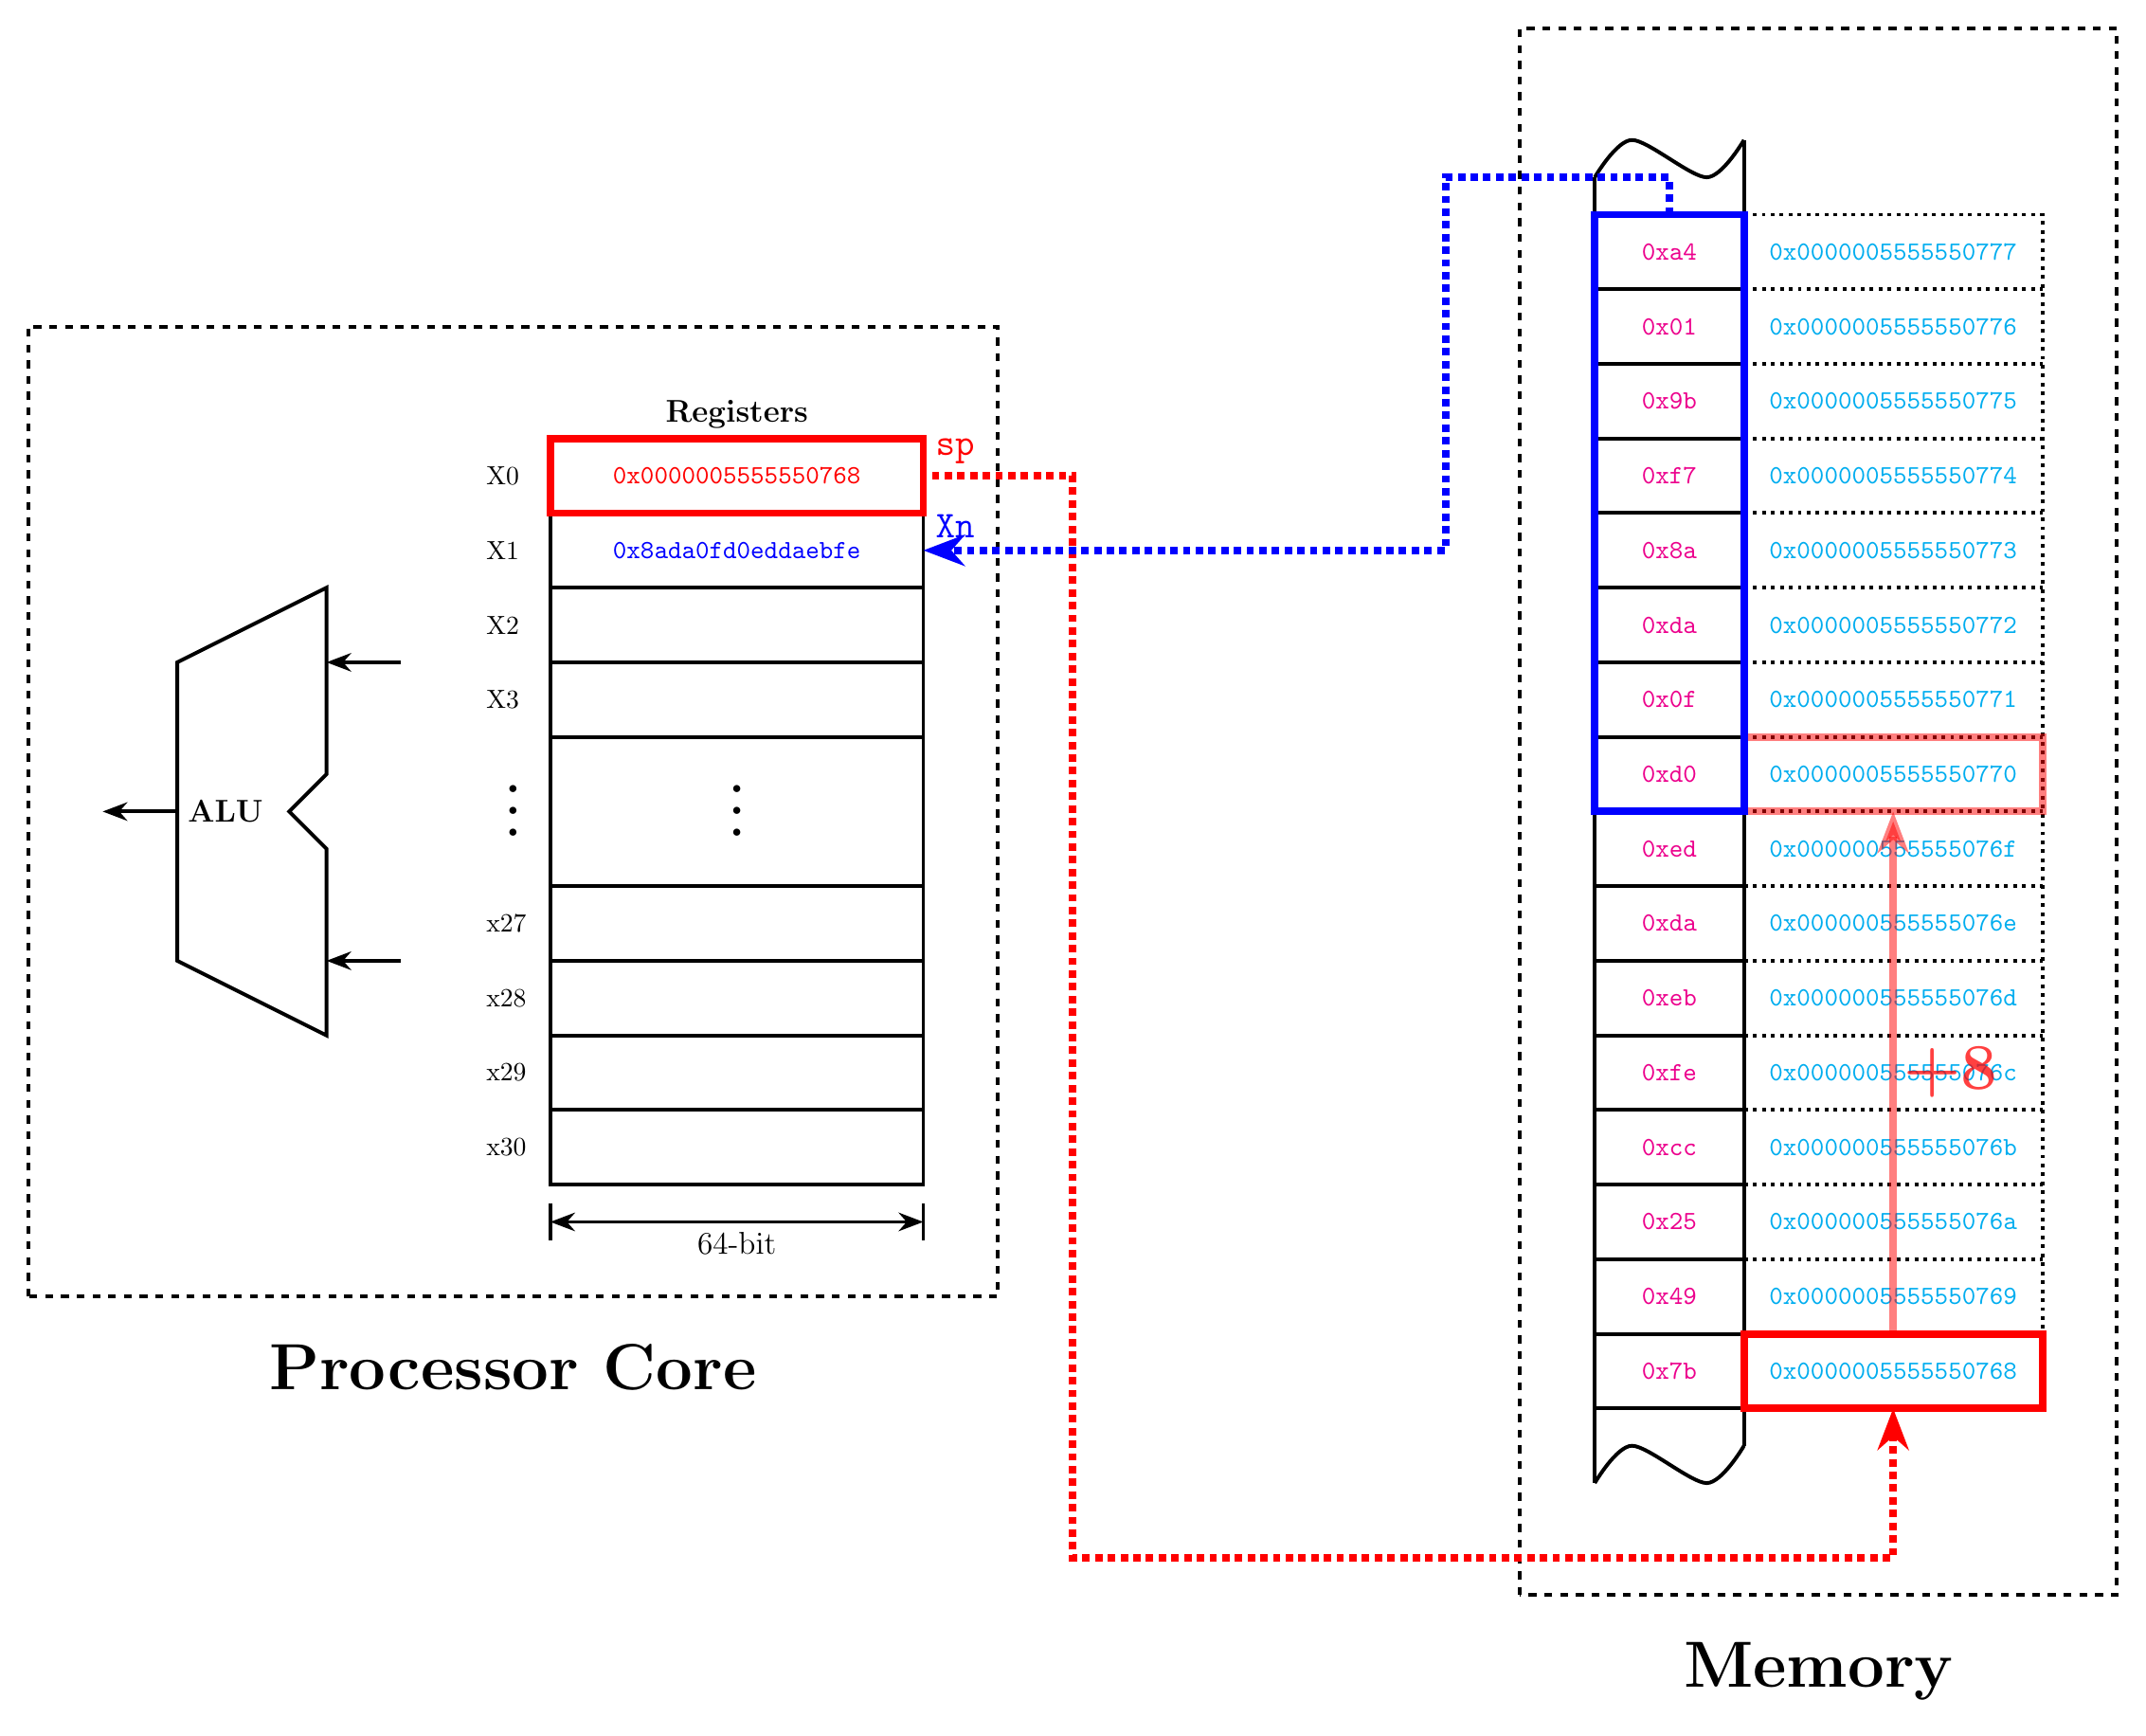
\begin{tikzpicture}[>=Stealth, line width=.5mm]
	\def \x{15}
	\def \y{15}
%	\draw[very thin,color=gray!15,step=.5] (-\x,-\y) grid (\x,\y);
%	
%	\foreach \i in {-\x,...,-2,-1,1,2,...,\x}
%	\draw[gray] (\i,.1)--(\i,-.1) node[below] {$\i$};%x-axis
%	\foreach \i in {-\y,-1,1,1,\y}
%	\draw[gray] (.1,\i)--(-.1,\i) node[left] {$\i$};%y-axis

% Processor Core Section
\begin{scope}[xshift=-2cm]
	% ALU Section (at x = -2)
	\draw[] (-10, -2) -- (-8, -3) -- (-8, -.5) -- (-8.5, 0) -- (-8, .5) -- (-8, 3) -- (-10, 2) -- cycle node[midway, right] {\large\bf ALU};
	\draw[->] (-10, 0) to (-11, 0);
	\draw[->] (-7, 2) to (-8, 2);
	\draw[->] (-7, -2) to (-8, -2);

	% Registers section (left side)
	\node[above] at (-2.5, 5) {\large\bf Registers};
	\draw[] (-5, -5) rectangle (0, 5); % Outer box
	\foreach \i in {0, 1, 2, 3} {
		\node[anchor=west] at (-6, 4.5-\i) {X\i};
	}
	\foreach \i in {27, 28, 29, 30} {
		\node[anchor=west] at (-6, -1.5-\i+27) {x\i};
	}
	\node[align=center,scale=.7] at (-5.5, 0) {$\bullet$\\ $\bullet$\\ $\bullet$};
	\node[align=center,scale=.7] at (-2.5, 0) {$\bullet$\\ $\bullet$\\ $\bullet$};
	\foreach \i in {4,3,2,1} {
		\draw (-5,\i) -- (0, \i);
		\draw (-5,-\i) -- (0, -\i);
	}
	\draw[] (-5, -5.25) to (-5, -5.75);
	\draw[] (0, -5.25) to (0, -5.75);
	\draw[<->] (-5, -5.5) to (0, -5.5);
	\node[below] at (-2.5, -5.5) {\large $64$-bit};
	\draw[dashed] (-12, -6.5) rectangle (1, 6.5);
	\node[below] at (-5.5, -7) {\Huge\bf Processor Core};
	
	\node[red] at (-2.5, 4.5) {\texttt{0x0000005555550768}};
	\node[blue] at (-2.5, 3.5) {\texttt{0x8ada0fd0eddaebfe}};
	
	\draw[red, line width=1mm] (-5, 4) rectangle (0, 5);
%	\draw[blue, line width=1mm] (-5, 1) rectangle (0, 2);
\end{scope}
	
% Memory section (right side)
\begin{scope}[xshift=7cm]
%	\node[magenta, above] at (1, 5) {\large\bf Contents};
%	\node[cyan, above] at (4, 5) {\large\bf Address};
	% Contents
	\draw[] (0, -8) rectangle (2, 8); % Outer box
	\draw[dotted] (2, -8) rectangle (6, 8); % Outer box
	\foreach \i in {7,6,...,0} {
		\draw (0,\i) -- (2, \i);
		\draw (0,-\i) -- (2, -\i);
	}
	% Address
	\foreach \i in {7,6,...,0} {
		\draw[dotted] (2,\i) -- (6, \i);
		\draw[dotted] (2,-\i) -- (6, -\i);
	}
	\draw (0,8) to (0,8.5); \draw (2,8) to (2,9);
	\draw[smooth] plot coordinates {(0,8.5) (.5, 9) (1.5, 8.5) (2,9)};
	\draw (0,-8) to (0,-9); \draw (2,-8) to (2,-8.5);
	\draw[smooth] plot coordinates {(2,-8.5) (1.5, -9) (.5, -8.5) (0,-9)};
	\draw[dashed] (-1, -10.5) rectangle (7, 10.5);
	\node[below] at (3, -11) {\Huge\bf Memory};
	
	\foreach \i/\j in {
		7.5/0xa4,
		6.5/0x01,
		5.5/0x9b,
		4.5/0xf7,
		3.5/0x8a,
		2.5/0xda,
		1.5/0x0f,
		.5/0xd0,
		-.5/0xed,
		-1.5/0xda,
		-2.5/0xeb,
		-3.5/0xfe,
		-4.5/0xcc,
		-5.5/0x25,
		-6.5/0x49,
		-7.5/0x7b
	} {
		\node[magenta] at (1, \i) {\texttt{\j}};
	}
	
	\foreach \i/\j in {
		7.5/0x0000005555550777,
		6.5/0x0000005555550776,
		5.5/0x0000005555550775,
		4.5/0x0000005555550774,
		3.5/0x0000005555550773,
		2.5/0x0000005555550772,
		1.5/0x0000005555550771,
		.5/0x0000005555550770,
		-.5/0x000000555555076f,
		-1.5/0x000000555555076e,
		-2.5/0x000000555555076d,
		-3.5/0x000000555555076c,
		-4.5/0x000000555555076b,
		-5.5/0x000000555555076a,
		-6.5/0x0000005555550769,
		-7.5/0x0000005555550768
	} {
		\node[cyan] at (4, \i) {\texttt{\j}};
	}

	\draw[red, line width=1mm] (2, -8) rectangle (6, -7);
	\draw[red, line width=1mm, opacity=.5] (2, 0) rectangle (6, 1);
	\draw[blue, line width=1mm] (0, 0) rectangle (2, 8);
	
	\draw[red, ->, line width=1mm, opacity=.5] (4,-7) to (4,0);
	\node[red, opacity=.75, right] at (4, -3.5) {\Huge\bf +8};
	
	\draw[dotted, red, line width=1mm, <-] (4, -8) -- (4,-10) -- (-7, -10) -- (-7, 4.5) -- (-9,4.5) node[above right] {\Large\ttfamily sp};
%	\draw[dotted, red, line width=1mm, <-, out=180, in=0] (2, -7.5) to (-9,4.5) node[above right] {\Large\ttfamily sp};
	\draw[dotted, blue, line width=1mm, ->] (1, 8) -- (1,8.5) -- (-2,8.5) -- (-2,3.5) -- (-9,3.5) node[above right] {\Large\ttfamily Xn};
\end{scope}
%\node[below] at (2.5,4) {\Huge\ttfamily ldr\hspace{1cm} x3, [x2]};
%\node[above] at (2.5,-5) {\Huge\ttfamily str\hspace{1cm} x3, [x2]};
\end{tikzpicture}
\end{document}
